\begin{frame}{Módulo \textit{Speech to Text}}{Requisitos}

\begin{itemize}
\item Em relação a reconhecimento de voz:
\begin{itemize}
  \item \textbf{Fluência}: Palavras conectadas
  \item<2-> \textbf{Dependência do usuário}: Sistema independente
  \item<3-> \textbf{Vocabulário}: Tipicamente pequeno
\end{itemize}

\item<4-> Execução do módulo em \textbf{paralelo} com o restante do jogo
\begin{itemize}
  \item Uso de uma \textit{thread}
\end{itemize}

\item<5-> Uso de um \textbf{\textit{buffer}} para armazenar palavras conforme são reconhecidas
\end{itemize}
\end{frame}

% ---------------------------------------------------------------------

\begin{frame}{Módulo \textit{Speech to Text}}{Implementação}

\only<1>{
\begin{figure}
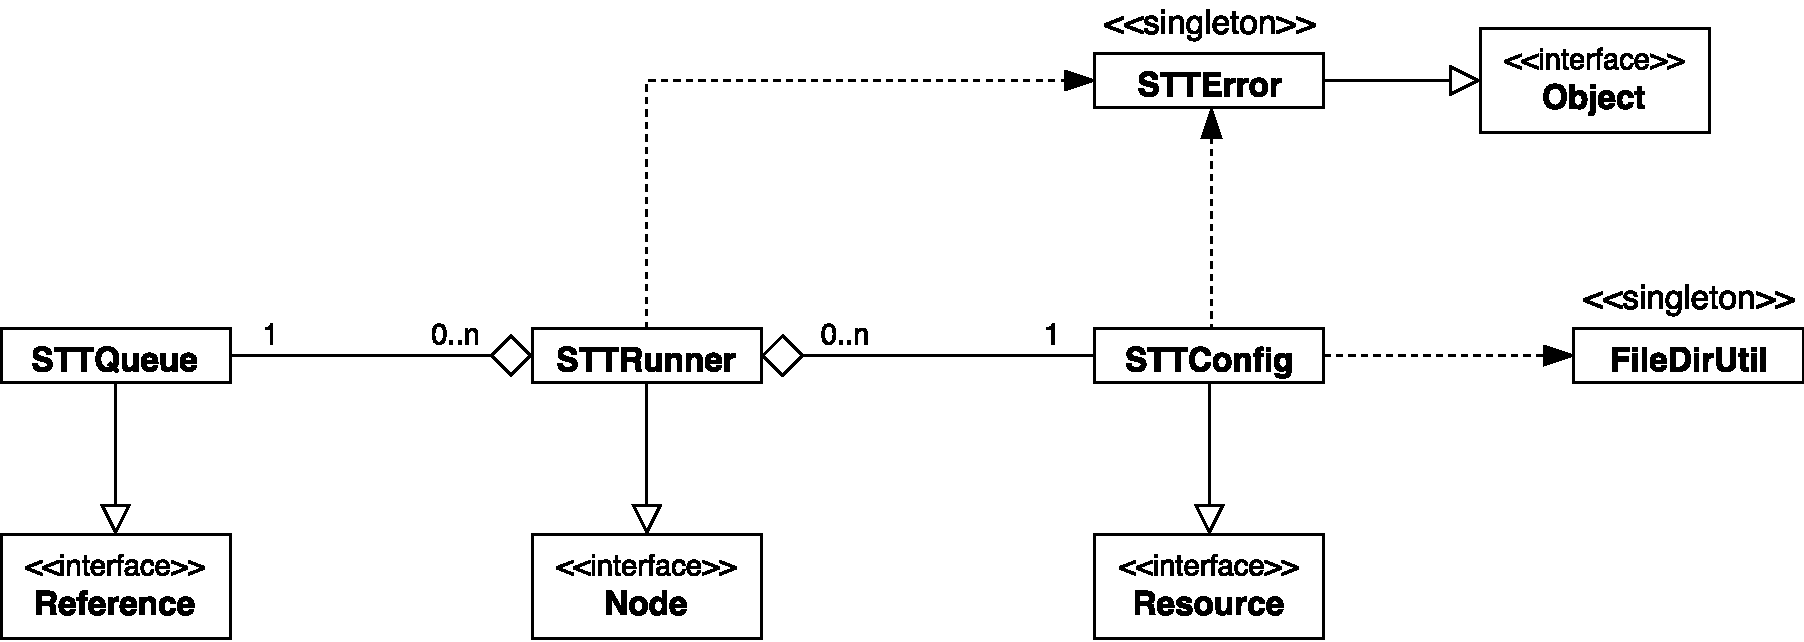
\includegraphics[width=.95\textwidth]{image/stt-module-simple.pdf}
\end{figure}
}

\only<2>{
\begin{figure}
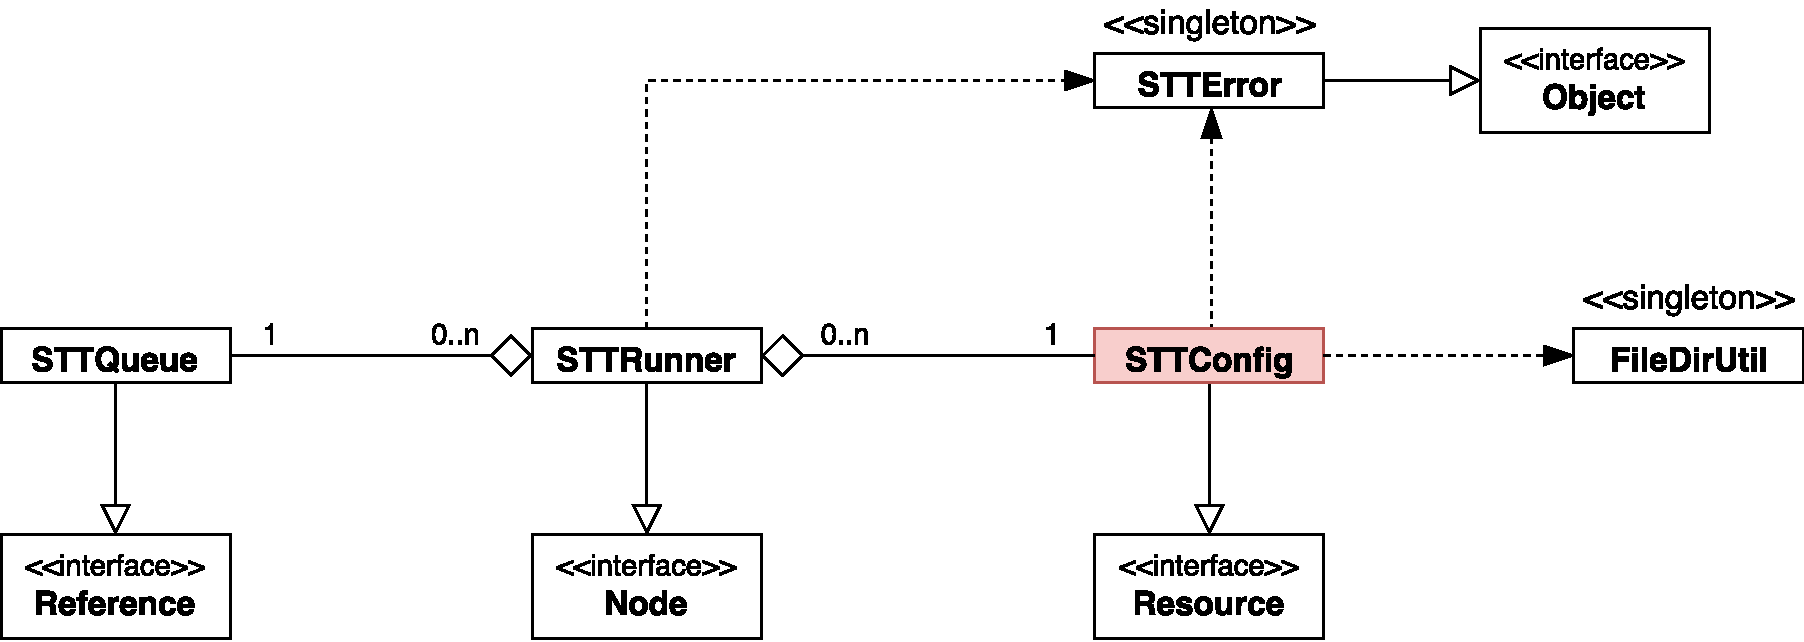
\includegraphics[width=.95\textwidth]{image/stt-module-sttconfig.pdf}
\end{figure}
}

\only<3>{
\begin{figure}
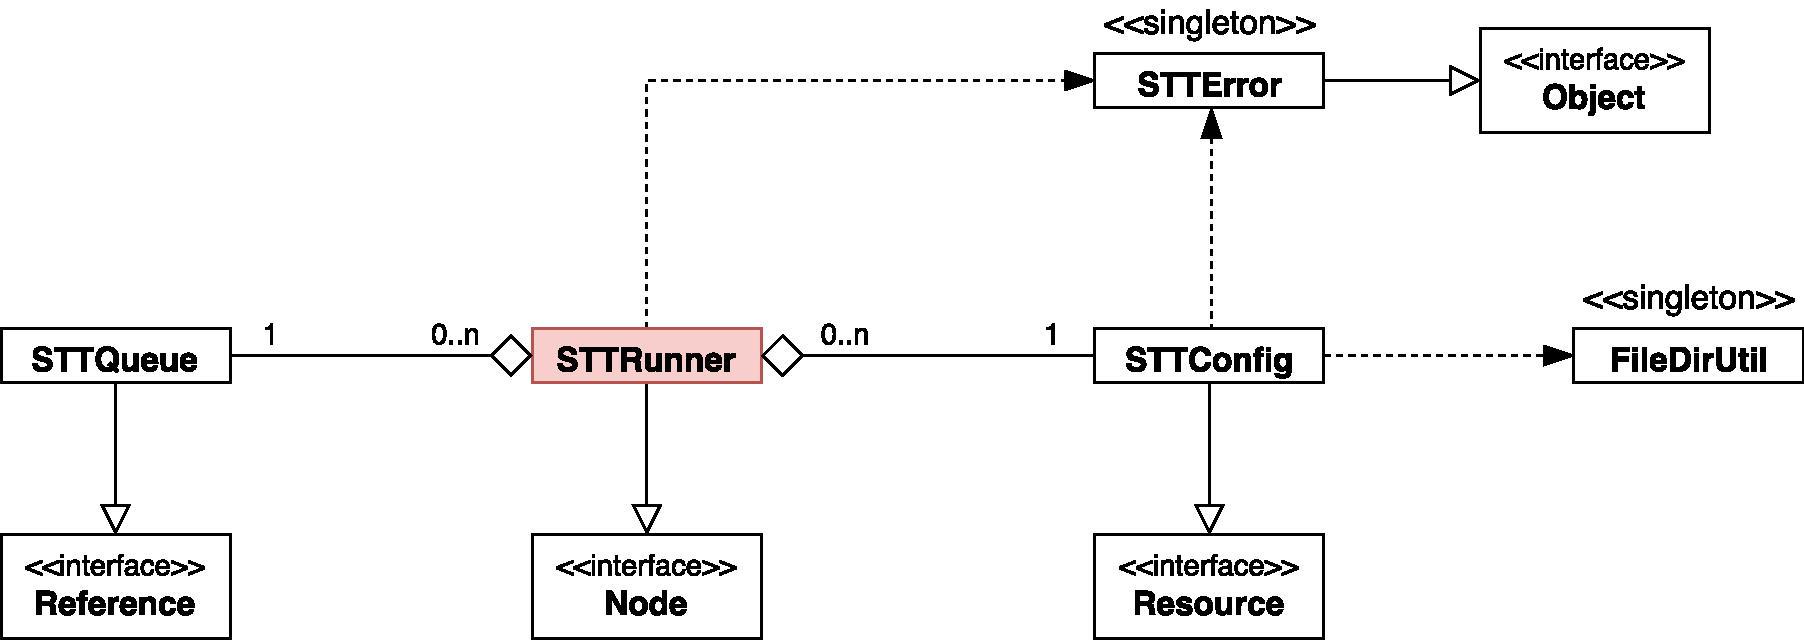
\includegraphics[width=.95\textwidth]{image/stt-module-sttrunner.pdf}
\end{figure}
}

\only<4>{
\begin{figure}
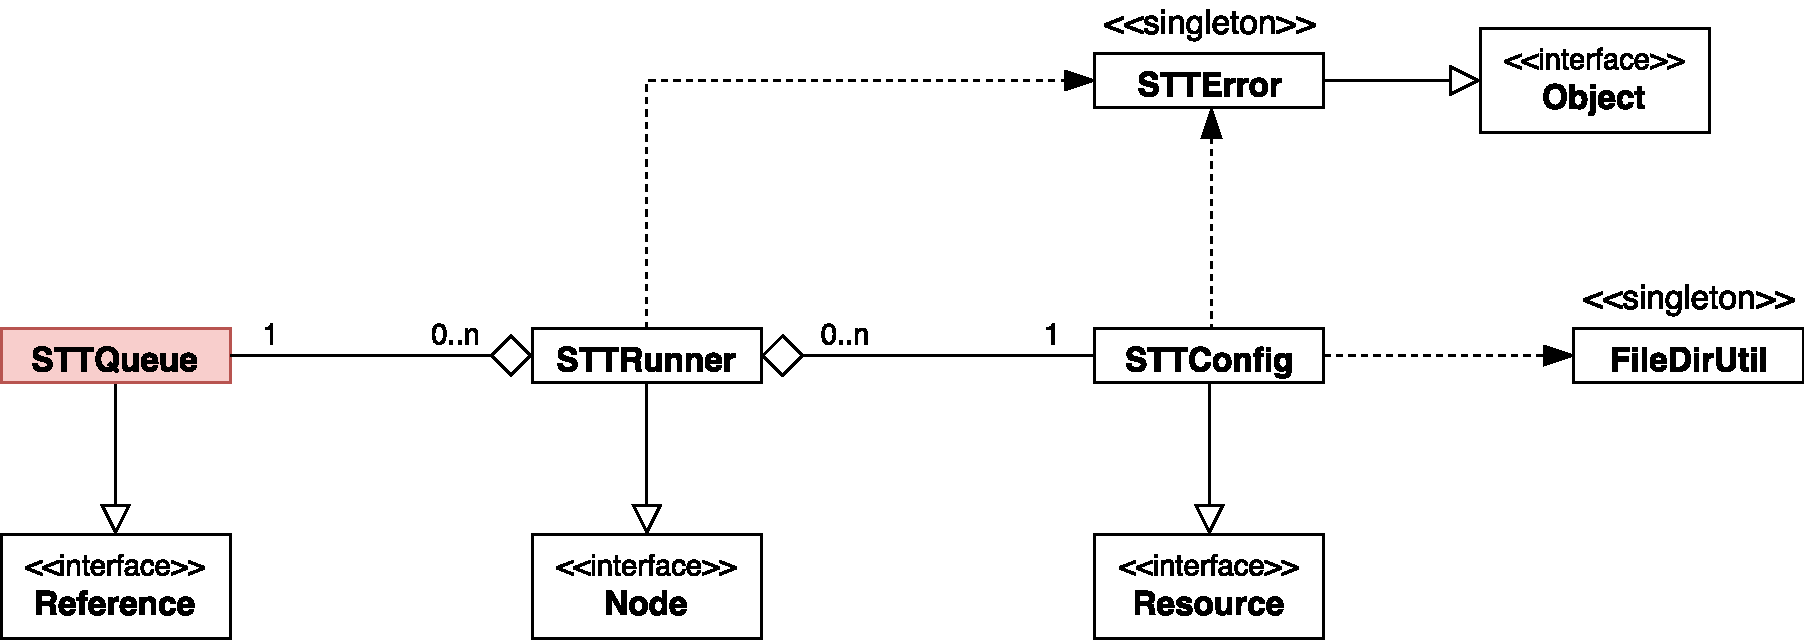
\includegraphics[width=.95\textwidth]{image/stt-module-sttqueue.pdf}
\end{figure}
}

\only<5>{
\begin{figure}
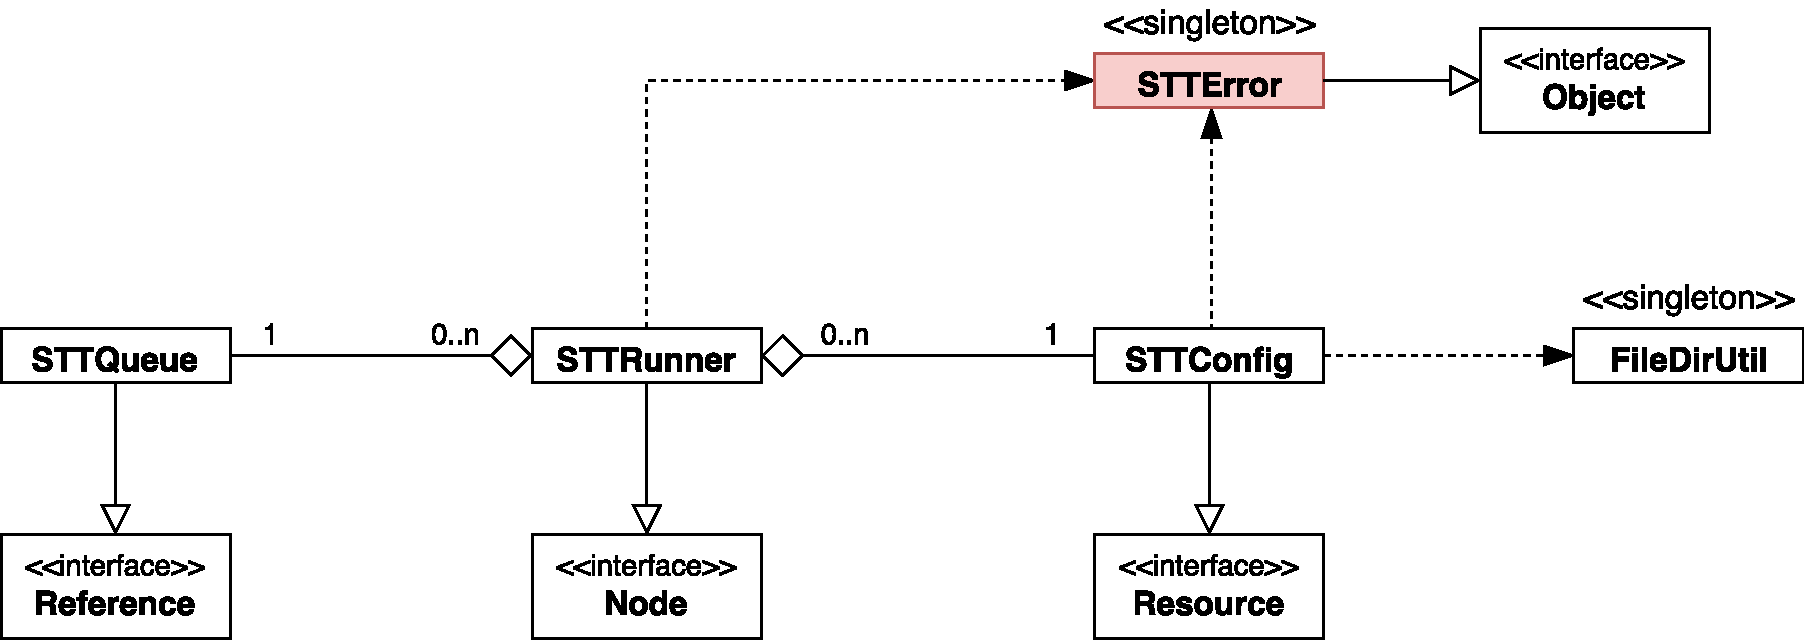
\includegraphics[width=.95\textwidth]{image/stt-module-stterror.pdf}
\end{figure}
}

\only<6>{
\begin{figure}
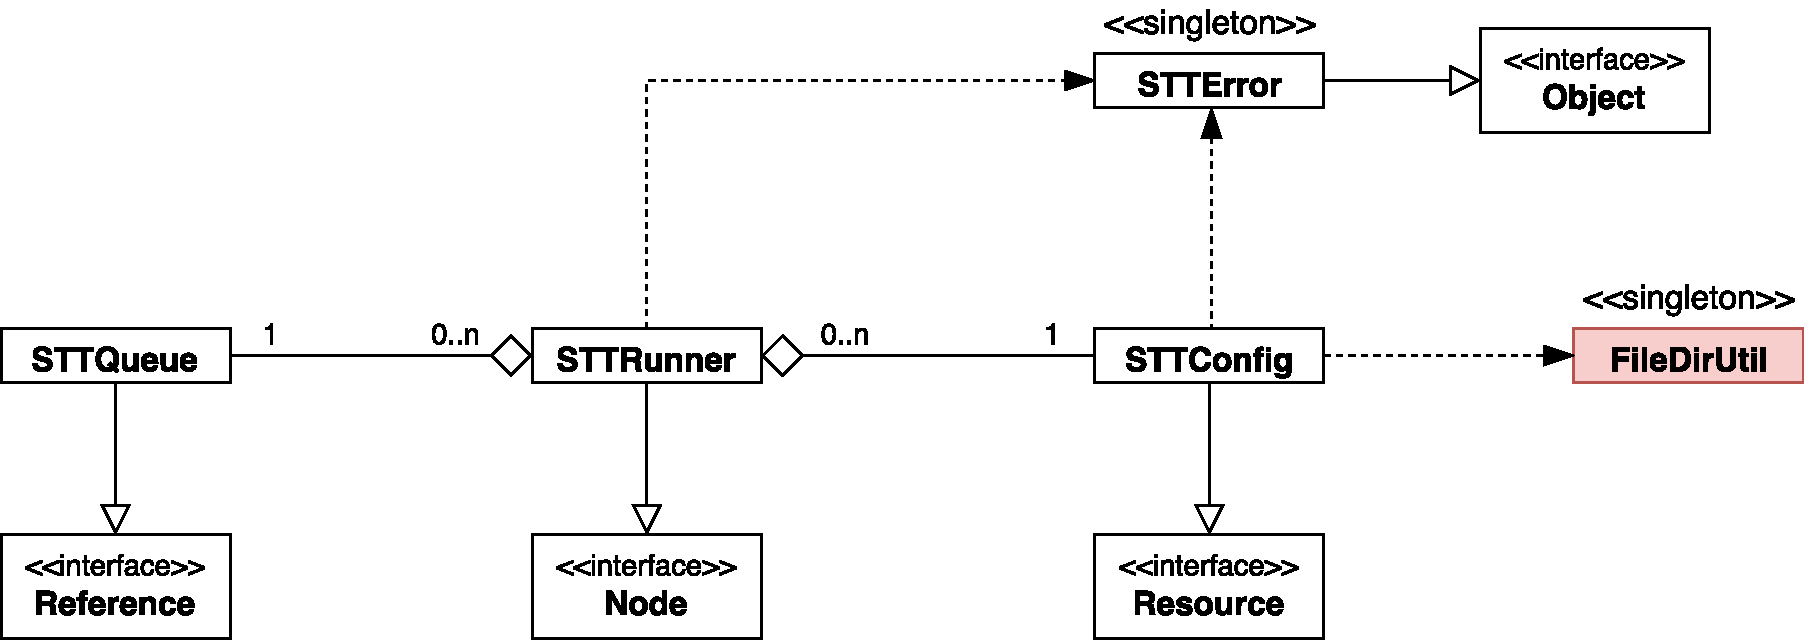
\includegraphics[width=.95\textwidth]{image/stt-module-filedirutil.pdf}
\end{figure}
}

\begin{itemize}
\item<2-> \texttt{STTConfig}: Controle dos arquivos de configuração
\item<3-> \texttt{STTRunner}: \textit{Thread} para realizar reconhecimento de voz
\item<4-> \texttt{STTQueue}: Fila para guardar palavras reconhecidas pelo \texttt{STTRunner}
\item<5-> \texttt{STTError}: Definição de constantes numéricas para possíveis erros
\item<6-> \texttt{FileDirUtil}: Classe auxiliar para manipular arquivos e diretórios
\end{itemize}

\end{frame}
